\documentclass[../thesis.tex]{subfiles}
\begin{document}

\chapter{Experiments}
\label{ch:experiments}
In this section, the frame field generation applied to a cube mesh
with some different metrics is discussed.
\emph{Setup:}
If not said otherwise, we run the frame field optimization to depth $3$ with $300$ diffusion steps.
We store the associated matrices of the metric field at each vertex of the
tet mesh. The cube has corners at $(0,0,0)$ and $(1,1,1)$.

To start, we apply the constant metric  $g^{1/2}=\mathrm{diag}(1,1,1)$
everywhere. The rotation coefficients $R$ are the identity matrix everywhere, as the metric does not twist or squish the space within the field.
The result is the boundary aligned frame field with no singularities, as the energy can be minimised to zero if the frames are constant. Figure \ref{fig:image1} shows the mesh used to store the metric
and the resulting constant frame field.
\begin{figure}[htb]
    \centering
    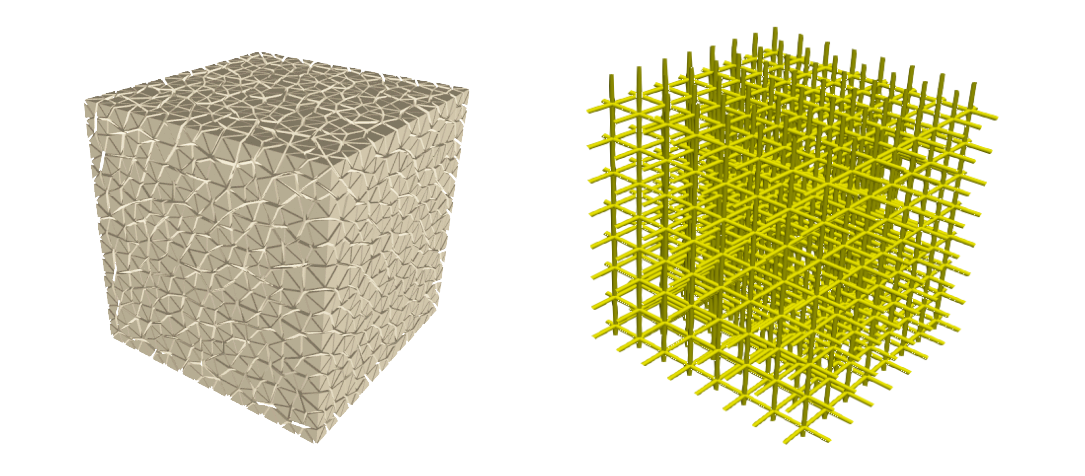
\includegraphics[width=\textwidth]{figures/image1}
    \caption{Left: The mesh used to store the metric field. Right: Constant metric everywhere which gives the boundary aligned constant frame field with no singularities.}
    \label{fig:image1}
\end{figure}

To further validate the frame field generation, we test a 2D analogue setup.
We divide the cube along
the $z$-axis into three equally sized parts.
Then, the metric varies only in the $x,z$-dimension.
The function to attach the metric to the vertices is defined as
\begin{equation}\label{eq:metric}
g^{1/2}(z) = \begin{cases}
    \mathrm{diag}(1,1,1) &0 < z < 1/3 \\
    \mathrm{diag}(h_k(z),1,h_k(z)) &1/3 < z < 2/3 \\
    \mathrm{diag}(k,1,k) &2/3 < z < 1 \\
\end{cases}\end{equation}
with $h_k(z)=3z(k-1)-k+2$.
The metric is constant in the $y$-axis and constant-linear-constant in the $x,z$-axis.
Thus, the rotation coefficients are only of the form
$$\begin{pmatrix}
    \cos (\alpha) & 0 & \sin(\alpha) \\
    0 & 1 & 0 \\
    -\sin(\alpha) & 0 & \cos(\alpha)
\end{pmatrix}$$
for some angle $\alpha$.
The result for a factor $k=10$ is depicted in figure \ref{fig:image2}.
\begin{figure}[htb]
    \centering
    \def\svgwidth{\textwidth}
    \input{figures/Zeichnung.pdf_tex}
    \caption{(a) The varying $g^{1/2}_{00}$ component along the $z$-axis for $k=10$. Visible is how
    the streamlines of the frame field only change in the middle third (b) and how the frames do not change along the $y$-axis (c).
    The singularities (d) are only points when taking a slice along the $y$-axis.}
    \label{fig:image2}
\end{figure}
For a factor of $k=10$,~4~singularities are present.
If we decrease the metric change in equation \ref{eq:metric} by
lowering the factor to $k=4$, less singularities are present (see figure \ref{fig:image3}).
\begin{figure}[htb]
    \centering
    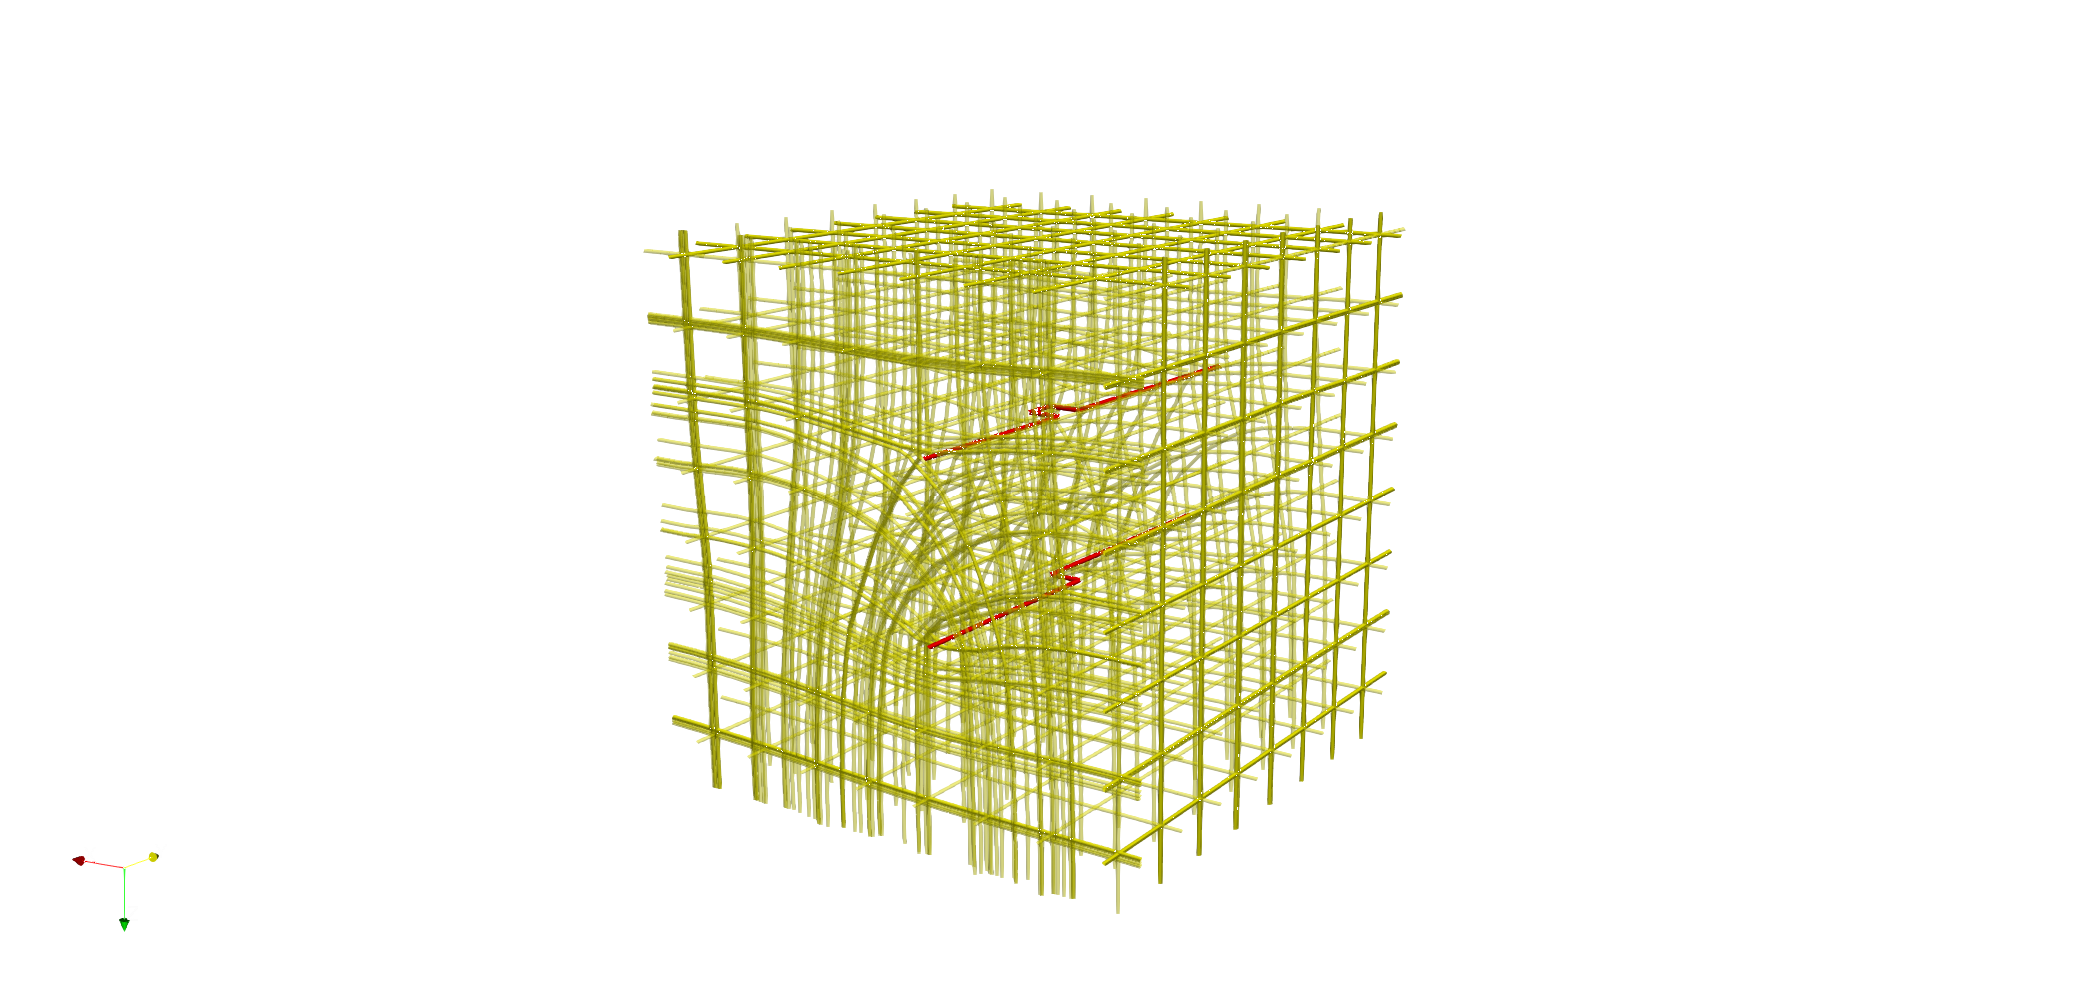
\includegraphics[width=25em]{figures/image3}
    \caption{With a lower factor of $k=4$, the metric change is not as extreme and less singularities are present.}
    \label{fig:image3}
\end{figure}
These results match with what previous works have done in 2D.
The third experiment shows how important higher depths (more subdivision of voxels) are.
Again, we divide the cube into three parts along the $z$-axis.
This time, we isotropically scale the metric, i.e. the metric is defined as
\begin{equation}\label{eq:isotropic} 
g^{1/2}(z) = \begin{cases}
    \mathrm{diag}(1,1,1) &0 < z < 1/3 \\
    \mathrm{diag}(h_k(z), h_k(z), h_k(z)) &1/3 < z < 2/3 \\
    \mathrm{diag}(k,k,k) &2/3 < z < 1 \\
\end{cases}.\end{equation}
We expect rotational symmetry (because the metric field is symmetric around the $z$-axis) of the singularity graph around the $z$-axis,
with the singularity structure going from side to side of the surface. We run the frame field optimization to different
depths, the result is pictured in figure \ref{fig:isotropic}. At depth 3 the singularities
cancel out before reaching the surface of the cube and do not connect in the middle. At depth 4, the singularity structure
looks better, but the arcs still cancel out before reaching the surface. At depth 5, it looks
the most reasonable, with the arcs reaching the surface and being connected in the middle.
However, it is still not perfect as we still expect a 90 degree rotational symmetry of the arcs.
An even higher depth is required, but due to the exponential time growth, this is not feasible
with the naive optimization approach. This fact further justifies only adaptively increasing resolution where is needed.
\begin{figure}[htb]
    \centering
    \def\svgwidth{\textwidth}
    \input{figures/isotropic.pdf_tex}
    \caption{The isotropic metric scaling from equation \ref{eq:isotropic} is run to different optimization depths.
    Depth 3 is lacking significant features of what we expect. At depth 4, the structure begins to look as expected, but e.g. still is not connected in the middle.
    At depth 5, it looks almost as expected. It does not quite show full 90 degree symmetry yet, as e.g. there is only one ``hook-arcs'' on the left, but two on the right of the cube.}
    \label{fig:isotropic}
\end{figure}
As a last example, we design a metric where we expect larger cubes at the surface of the cube and smaller in the interior.
We divide the cube into 3 parts, but this time from the center out.
We measure the radius to the center of the cube with the infinity-norm.
In the inner third of the cube, we set $g^{1/2}=\mathrm{diag}(1,1,1)$.
The metric is linearly increasing to $k=10$ in the second third
and in the outside third, it is a constant metric again at $g^{1/2}=\mathrm{diag}(10,10,10)$.
We expect pointwise symmetry of the singularity graph around the center of the cube.
The result is shown in figure \ref{fig:nonuniform}. 
\begin{figure}[htb]
    \centering
    \def\svgwidth{25em}
    \input{figures/nonuniform.pdf_tex}
    \caption{Left: The nonuniform metric, visualized is the $g_{00}^{1/2}$ component. Right: The singularity graph.
    The optimization is run to depth 5. Lower depths displayed similar defects as described in figure~\ref{fig:isotropic}, where
    the singularity structure was not fully formed yet.}
    \label{fig:nonuniform}
\end{figure}

\end{document}